
\documentclass[ignorenonframetext]{beamer}
\usetheme{sts}
\title[Learning for probabilistic timed automata]{Incremental Measurement of Model Similarities in Probabilistic Timed Automata Learning}

\usepackage{graphicx}
\usepackage{natbib}
\usepackage{subfig}
\usepackage{outlines}
\usepackage{multicol}
\usepackage{tikz-uml}
\usepackage{physics}
\usepackage{tikz}
\usepackage{algorithm}
\usepackage{algpseudocode}  
\usetikzlibrary{matrix}
\captionsetup{font=scriptsize}
\captionsetup[figure]{labelformat=empty}

\author{Salvador Fernandez Covarrubias}
\institute{Institute for Software Systems}
\date{\today}

\begin{document}
\begin{document}
	\begin{frame}<presentation>[plain]
	\titlepage{}
\end{frame}

\begin{frame}<presentation>
\frametitle{Objective}
\begin{itemize}
	\item Learning, measuring and modelling observations of probabilistic timed automata \textit{on-the-fly}, applying the following concepts:
	\begin{itemize}
		\item Passive learning of observations, by fitting the curve of the data to mathematical equations.
		\item Incremental measurement and modelling of observations, based on Euclidean distances and cost functions. 
		\item Model similarity evaluations, utilizing graph matching techniques.
	\end{itemize}
\end{itemize}
\end{frame}

\begin{frame}<presentation>
\frametitle{Objective}
\centering
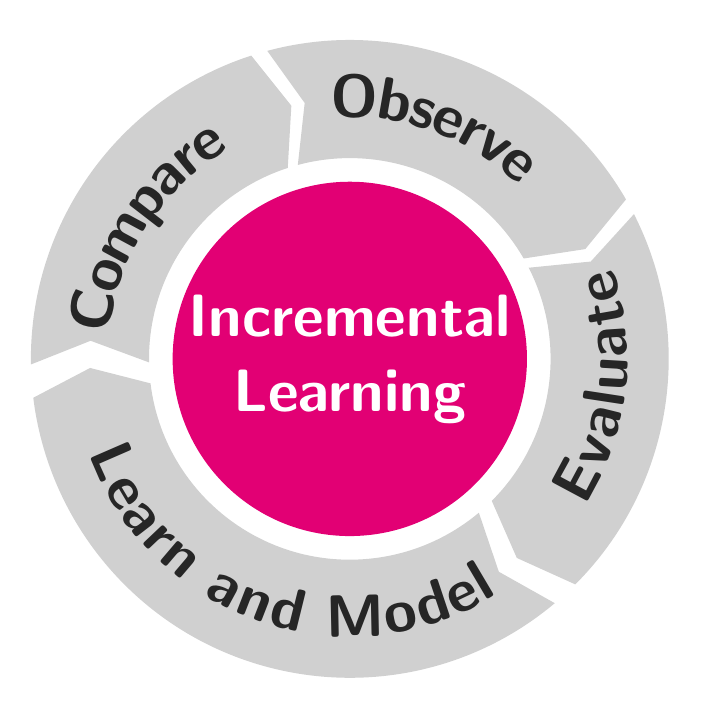
\includegraphics[scale=0.5]{./pictures/motivation2.png}
\end{frame}

\begin{frame}<presentation>
\frametitle{Contents}
\tableofcontents[]{}
\end{frame}

\section{Timed Automata}

\begin{frame}
\frametitle{Timed Automata}
\theoremstyle{definition}
\scriptsize
\begin{definition}{}
	A timed automaton $A$ is a tuple $< L , L_{0}, \Sigma ,X, I, E >$ where,
\end{definition}
\begin{itemize}
	\item[--]
	$L$ is a finite set of locations.
	\item[--]
	$L_{0}$ is the initial location, $L_{0}\in L$.
	\item[--]
	$\Sigma$ is a finite set called the alphabet or also actions from $A$. 
	\item[--]
	$X$ is a finite set of clocks. 
	\item[--]
	$I$ labels each location with some clock constraint $\Phi (X)$, which represents a mapping from $X$ to the set $\mathbb{R}$ of non-negative real numbers. 
	\item[--]
	$E \subseteq L \times \Sigma \times 2^{X} \times \Phi (x) \times L$ is a set of transitions. A transition $\langle l,a,\varphi, \lambda, l' \rangle$  represents an edge from a location $l$ to location $l'$ given an action $a \in \Sigma$, $\varphi \in \Phi (x)$ is a clock constraint over $X$ that specifies when a transition is enabled, and $\lambda \subseteq X$ represent a clock reset function. 
\end{itemize}
\end{frame}

\section{UPPAAL}

\begin{frame}
\frametitle{UPPAAL - Models}
\scriptsize
\begin{itemize}
	\item UPPAAL is a tool for modeling, simulating and verifying real-time systems. Nevertheless, we only use it to model and simulate probabilistic timed automata.
	\item Locations are identified by labels and can be bound to invariants, which may allow time to elapse while a location remains idle.
	\item Edges represent transitions and may be composed of guards, actions or assignments; where guards represent a condition that an edge must satisfy.
	\item Branch points allow automata to choose transitions non-deterministically, by assigning weighted-probability values to edges.  
\end{itemize}
%
\begin{center}
	\includegraphics[scale=0.5]{./Pictures/uppaal_model_example.PNG}
\end{center}
%
\end{frame}

\begin{frame}
\frametitle{UPPAAL - Simulations}
\begin{itemize}
	\item UPPAAL provides a query language that allows to visualize the values of expressions along simulated runs. The syntax of the queries is as follows: \newline
	 \begin{equation*}
	simulate \; N \; [<=bound] \; \{E1, \dots, Ek\}
	\end{equation*}
	\item where $N$ is a natural number indicating the number of simulations to be performed, $bound$ is the time bound of the simulations, and $\{E1, \dots, Ek\}$ are the expressions that are to be monitored. 
\end{itemize}

\end{frame}

\begin{frame}
\frametitle{Example}
\centering
\begin{center}
	\begin{figure}
		\includegraphics[scale=0.3]{./Pictures/uppaal_model_example.PNG}
		\caption{Observed Model}
	\end{figure}
	\begin{figure}
		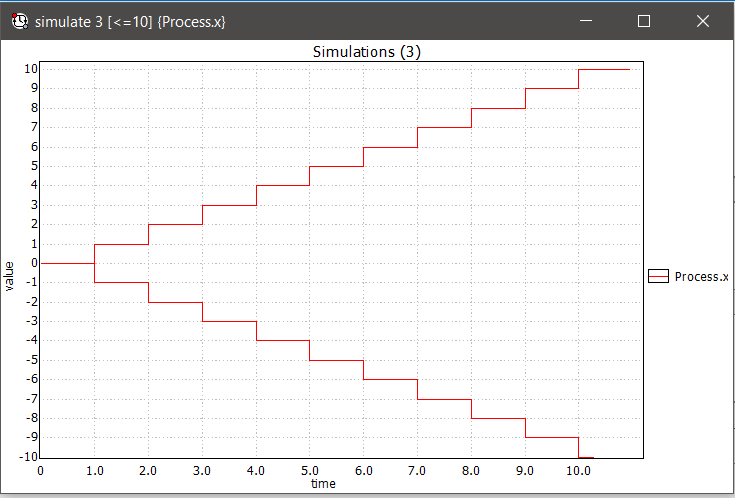
\includegraphics[scale=0.3]{./Pictures/uppaal_model_example_simulation.PNG}
		\caption{Simulation: \textit{simulate 3 [$\leq$ 10] Process.x}}
	\end{figure}
%	\includegraphics[scale=0.4]{./Pictures/uppaal_model_example.PNG}
%	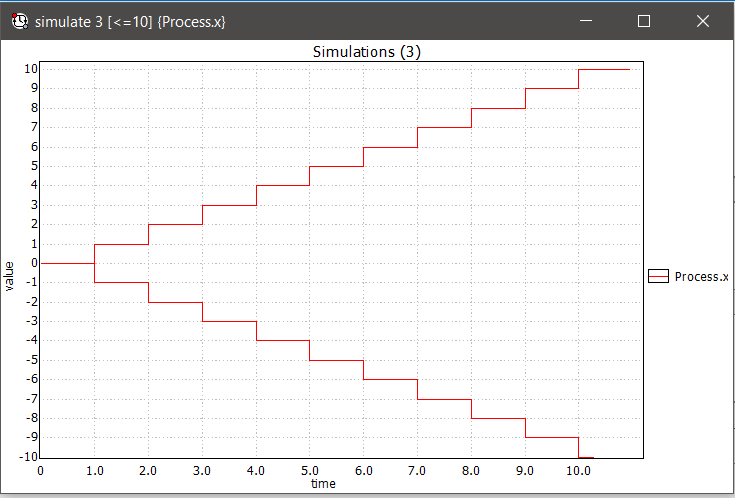
\includegraphics[scale=0.3]{./Pictures/uppaal_model_example_simulation.PNG}
\end{center}
\end{frame}

\begin{frame}
\frametitle{Data Fitting}
\begin{itemize}
	\small
	\item We consider an observation as the value of a variable in an exact time, obtained from
	a simulation run.
	\item Gathering more than one observation and fitting the curve of
	the data, allows us to derive equations that express the behavior of a variable given
	a period of time.
	\item A simulation run is a set of observations that are transformed to a set of equations.  
\end{itemize}

\begin{center}
	\tiny
	\begin{tabular}{||c c c ||}
		\hline
		Observation & Time & Value \\ [0.5ex] 
		\hline\hline
		1 & 0 & -1 \\ 
		\hline
		2 & 1 & -2 \\
		\hline
		3 & 2 & -3 \\
		\hline
		4 & 3 & -4 \\
		\hline
		5 & 4 & -5 \\
		\hline
		6 & 5 & -6 \\
		\hline
		7 & 6 & -7 \\
		\hline
		8 & 7 & -8 \\
		\hline
		9 & 8 & -9 \\
		\hline
		10 & 9 & -10 \\ [1ex] 
		\hline
	\end{tabular}
\end{center}

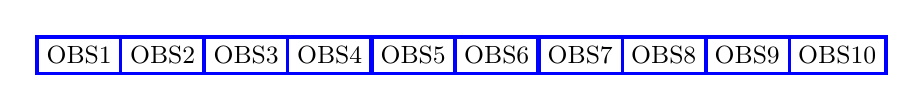
\begin{tikzpicture}
\tikzset{
	mstyle/.style={column sep=-\pgflinewidth,nodes={draw},font=\small},
	window/.style={draw,very thick,blue},
}
\matrix(m)[matrix of nodes,ampersand replacement=\&,mstyle]{
	OBS1 \& OBS2 \& OBS3 \& OBS4 \& OBS5 \& OBS6 \& OBS7 \& OBS8 \& OBS9 \& OBS10 \\
};
\foreach \j [count=\i] in {4,...,10}{
	\onslide<\i>{
		\draw[window](m-1-\i.north west)rectangle(m-1-\j.south east);
}}
\end{tikzpicture}

\begin{itemize}
	\small
	\item $x=x-1$ from times \only<1>{0-3}\only<2>{0-4}\only<3>{0-5}\only<4>{0-6}\only<5>{0-7}\only<6>{0-8}\only<7>{0-9}
\end{itemize}

\end{frame}

\section{Incremental Learning}

\begin{frame}
\frametitle{Data Learning and Measurement}
\framesubtitle{Data Learning}
\small
\begin{itemize}
	\item An equation trace is a list of mathematical equations organized in chronological order, that represent the behavior of a simulation run from an observed automaton.  
	\item The learned model \textit{lm} represents the learned automaton, which is created based on the equations derived from the observations. 
\end{itemize}
%
\centering
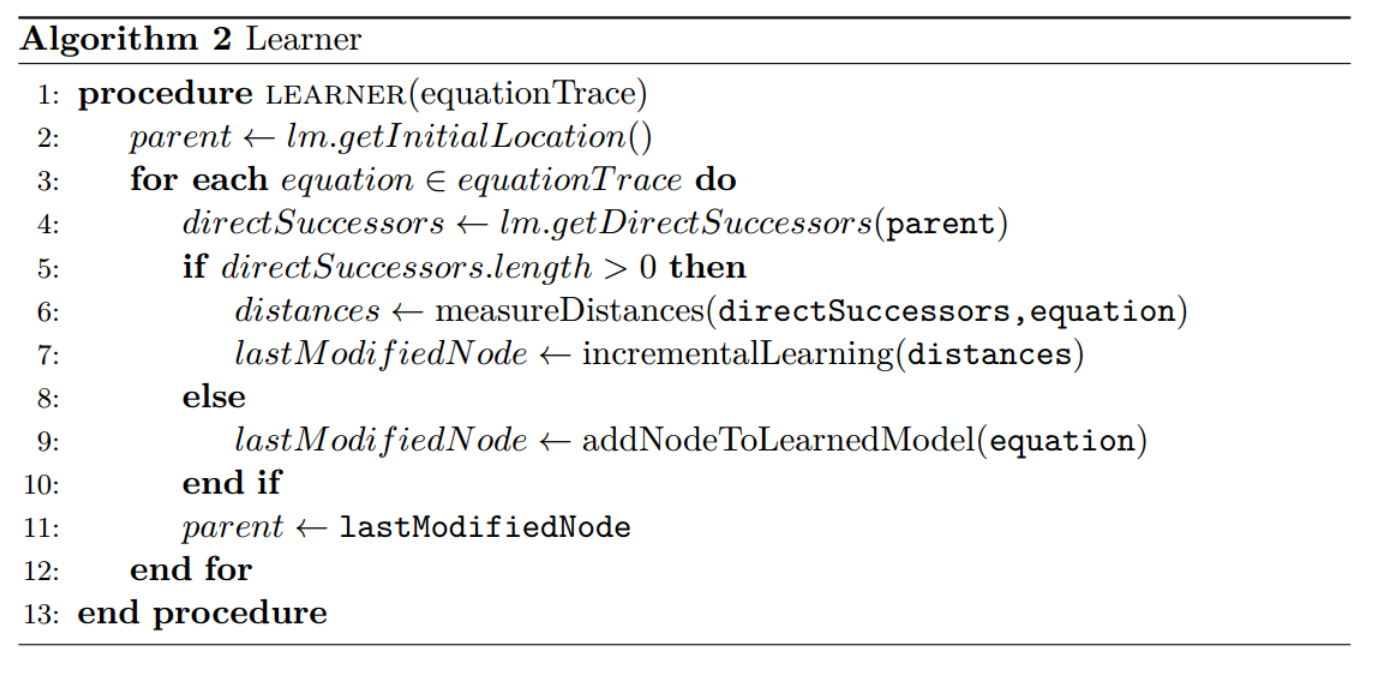
\includegraphics[scale=0.3]{./pictures/learner_algorithm.png}
%
\end{frame}

\begin{frame}
\frametitle{Data Modeling} 
%\framesubtitle{Data Measurement}
\small
\begin{itemize}
	\item Assuming that we derived the following equation list from the data of a simulation run:
	\begin{itemize}
		\item  $EQ1 \rightarrow x=x+5,$ $time \rightarrow (0s-15s)$
		\item  $EQ2 \rightarrow x=x+6,$ $time \rightarrow (15s-30s)$
		\item  $EQ3 \rightarrow x=x+10,$ $time \rightarrow (30s-45s)$
	\end{itemize}
	\item Learned Model (\textit{lm}): 
	\begin{center}
		\only<1>{
			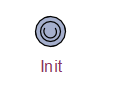
\includegraphics[scale=0.4]{./pictures/recreation_example/model_part1.png}
		}
		\only<2>{
			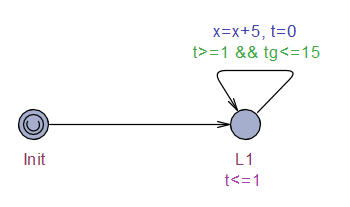
\includegraphics[scale=0.4]{./pictures/recreation_example/model_part2.png}
		}
		\only<3>{
			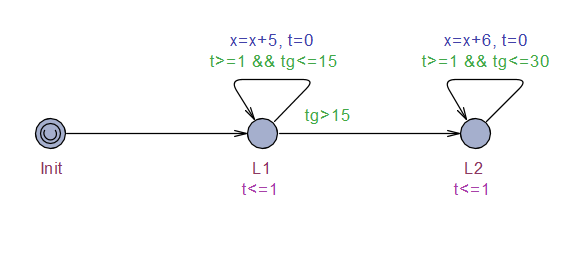
\includegraphics[scale=0.4]{./pictures/recreation_example/model_part3.png}
		}
		\only<4>{
			\includegraphics[scale=0.4]{./pictures/recreation_example/learned_model_example.png}
		}
		\only<5>{
			\includegraphics[scale=0.4]{./pictures/recreation_example/learned_model_example.png}
			\item What happens when we derive different equations in other simulation runs? For example: $EQ1 \rightarrow x=x+1,$ $time \rightarrow (0s-10s)$
		}
	\end{center}
	
\end{itemize}

\end{frame}

\begin{frame}
\frametitle{Data Learning and Measurement}
\framesubtitle{Data Measurement}
%\tiny
%\begin{itemize}
%	\item Euclidean distance
%\end{itemize} 
%
\centering
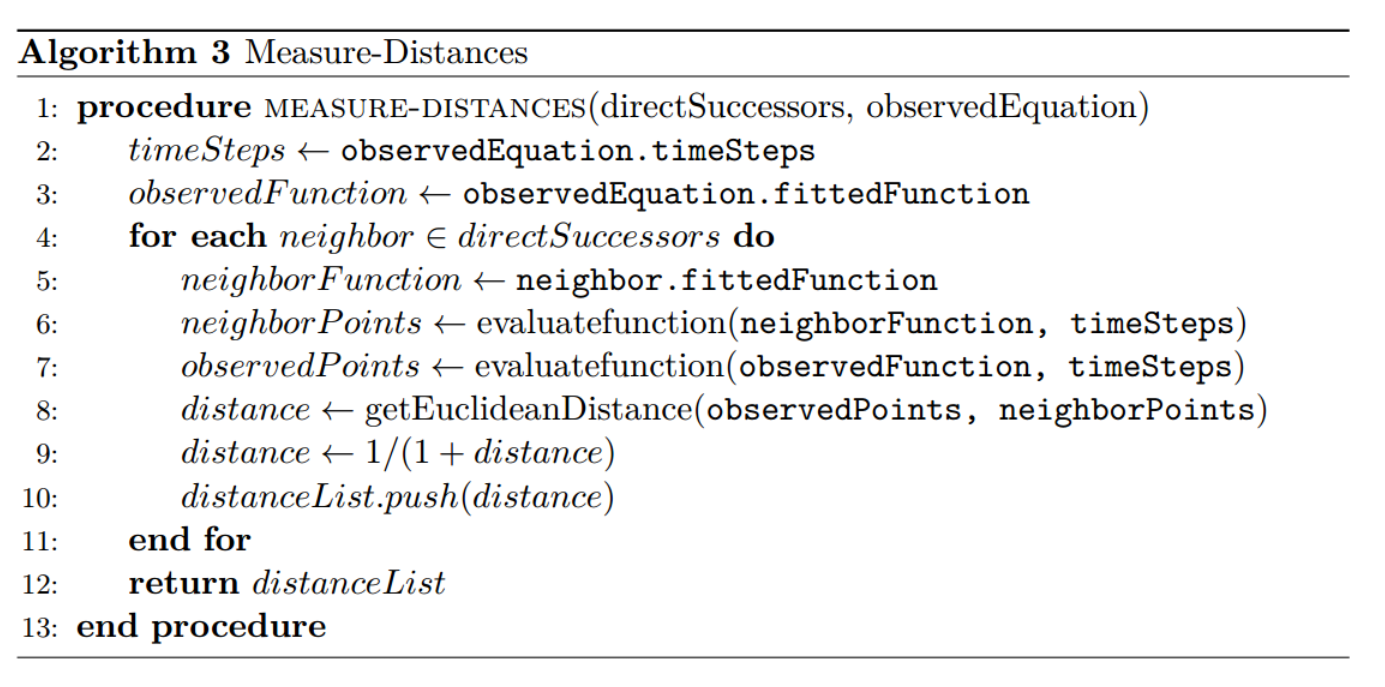
\includegraphics[scale=0.4]{./pictures/measure_distances_algorithm.png}
%
\end{frame}

\begin{frame}
\frametitle{The Cost Function}
\scriptsize
\begin{itemize}
	\item The closest distance among all direct successors (if any) is chosen. 
		\begin{align*} 
		Cost  =  nodeCount * nodeCost &+ propagation_f * functionalityCost  \\ 
		& + propagation_t * timeCost
		\end{align*}
	\item Important to notice that every cost may or may not be the same, and that we always consider the lowest cost as the best option. 
\end{itemize}
\centering
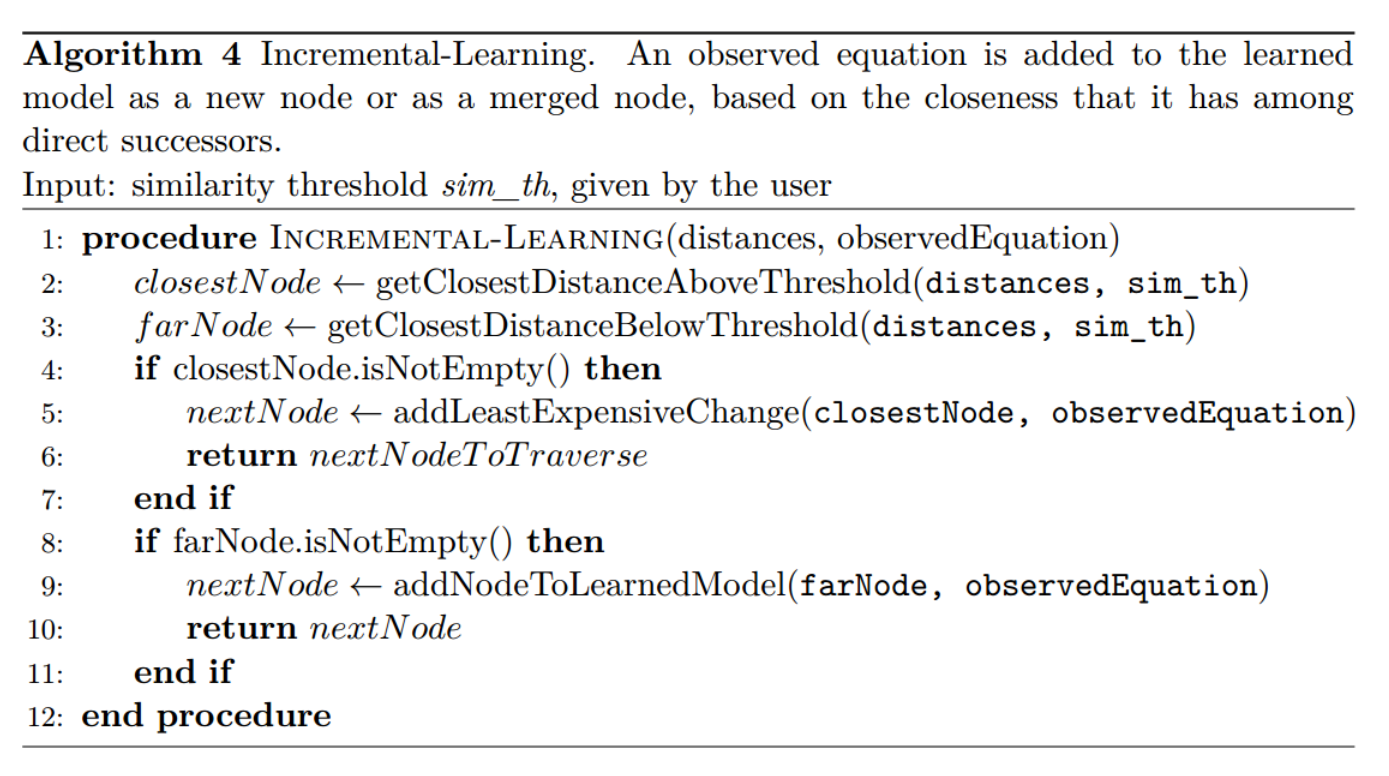
\includegraphics[scale=0.3]{./pictures/incremental_learner_algorithm.png}
\end{frame}

\begin{frame}
\frametitle{Node Addition Cost}
\tiny
\begin{itemize}
	\item Assuming the following observation: $EQ1 \rightarrow x=x+1,$ $time \rightarrow (0s-10s)$
	\item No functionality from the model is modified, but an extra location is added. 
	\item $Cost  =  nodeCount * nodeCost$. 
\end{itemize}
\begin{figure}
	\includegraphics[scale=0.28]{./pictures/learned_model_example.png}
	\caption{Learned Model}
\end{figure}
\begin{figure}
	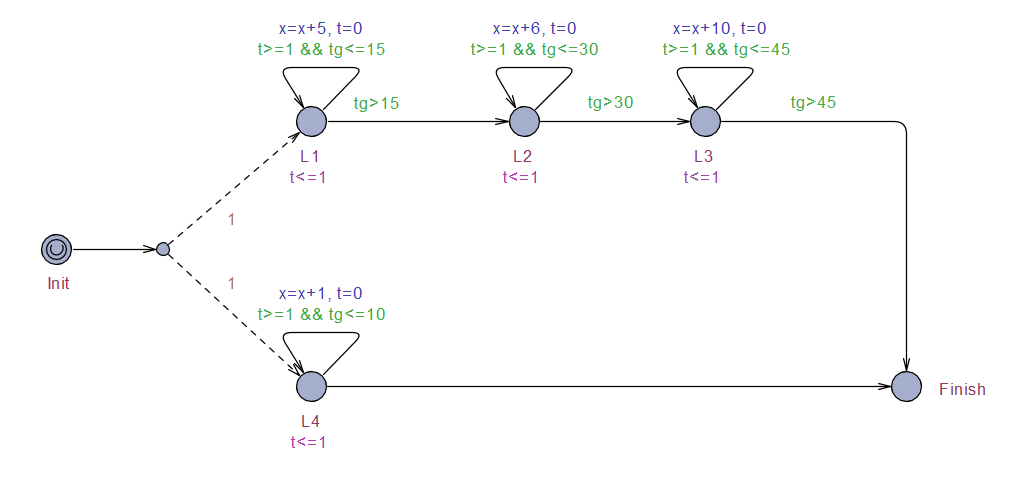
\includegraphics[scale=0.28]{./pictures/learned_model_example_addition.png}
	\caption{Learned Model After Addition}
\end{figure}
\end{frame}

\begin{frame}
\frametitle{Node Replacement Cost}
\tiny
\begin{itemize}
	\item Assuming the following observation: $EQ1 \rightarrow x=x+1,$ $time \rightarrow (0s-10s)$
	\item Functionalities and time constraints of locations may be modified.
	\item $Cost = propagation_f * functionalityCost + propagation_t * timeCost$, where
	$propagation_f$ is the distance of the old functionality $x=x+5$ and the new functionality $x=x+3$, and $propagation_t$ the difference of time constrains in terms of second (e.g. 5 seconds). 
\end{itemize}
\begin{center}
	\begin{figure}
		\includegraphics[scale=0.35]{./pictures/learned_model_example.png}
		\caption{Learned Model}
	\end{figure}
	\begin{figure}
		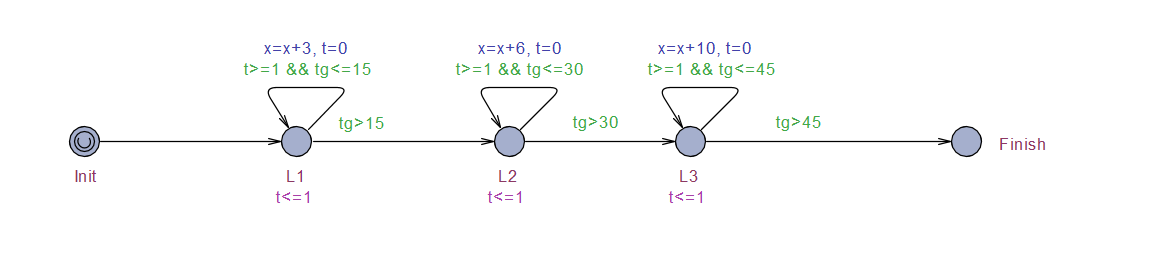
\includegraphics[scale=0.35]{./pictures/learned_model_example_replacement_functionality.png}
		\caption{Learned Model After Replacement}
	\end{figure}
\end{center}
\end{frame}

%\begin{frame}
%\frametitle{Node Replacement Cost}
%\tiny
%\begin{itemize}
%	\item Assuming the following observation: $EQ1 \rightarrow x=x+1,$ $time \rightarrow (0-10s)$
%	\item Locations may also be added. 
%	\item $Cost = nodeCount * nodeCost + propagation_t * timeCost$. 
%\end{itemize}
%\begin{center}
%	\begin{figure}
%		\includegraphics[scale=0.4]{./pictures/learned_model_example.png}
%		\caption{Observed Model}
%	\end{figure}
%	\begin{figure}
%		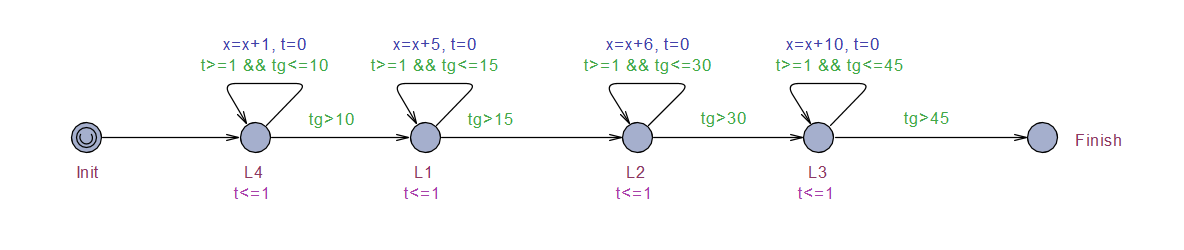
\includegraphics[scale=0.4]{./pictures/learned_model_example_time_replacement_addition.png}
%		\caption{Learned Model}
%	\end{figure}
%\end{center}
%\end{frame}

\begin{frame}
\frametitle{Model Similarities Comparison}
%
\begin{center}
\small
\only<1>{
	The goal is to match the nodes and edges of two automata. 
%	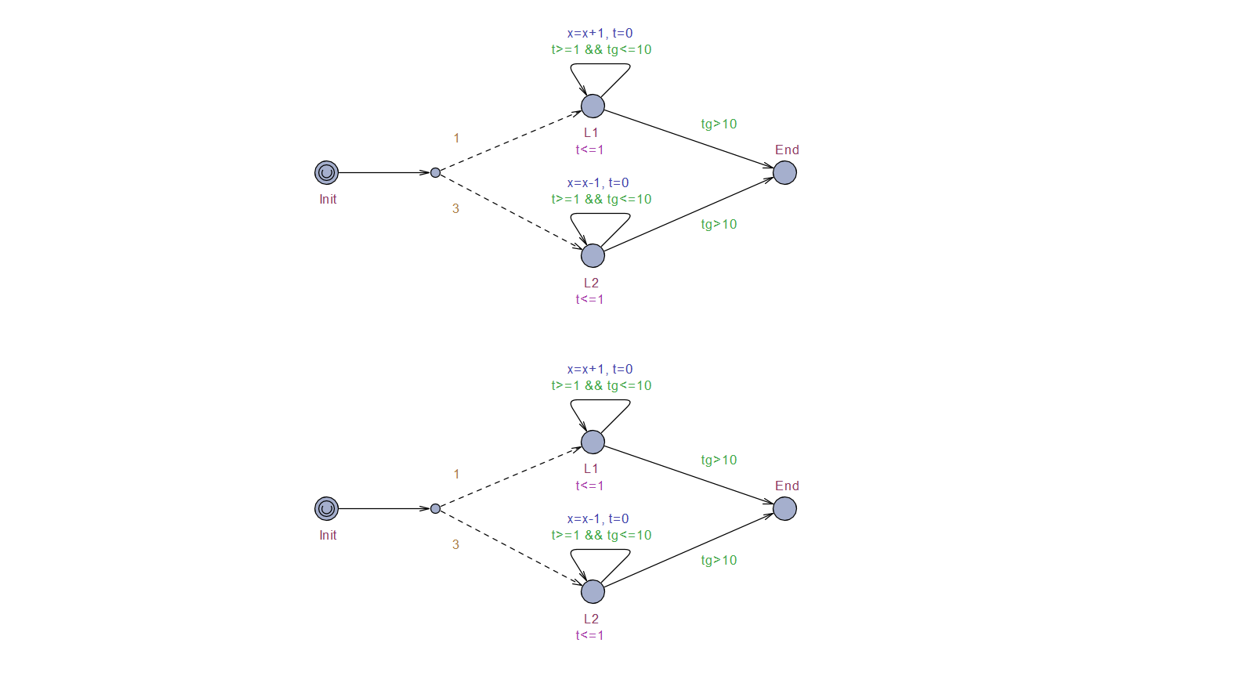
\includegraphics[scale=0.4]{./pictures/model_comparison/step1.png}
\begin{figure}
	\includegraphics[scale=0.28]{./pictures/model_comparison/uppaal_model_example.png}
	\caption{Observed Model}
\end{figure}
\begin{figure}
	\includegraphics[scale=0.28]{./pictures/model_comparison/uppaal_model_example.png}
	\caption{Learned Model}
\end{figure}

}
\only<2>{
	We first strip the labels of the learned model. 
\begin{figure}
	\includegraphics[scale=0.28]{./pictures/model_comparison/uppaal_model_example.png}
	\caption{Observed Model}
\end{figure}
\begin{figure}
	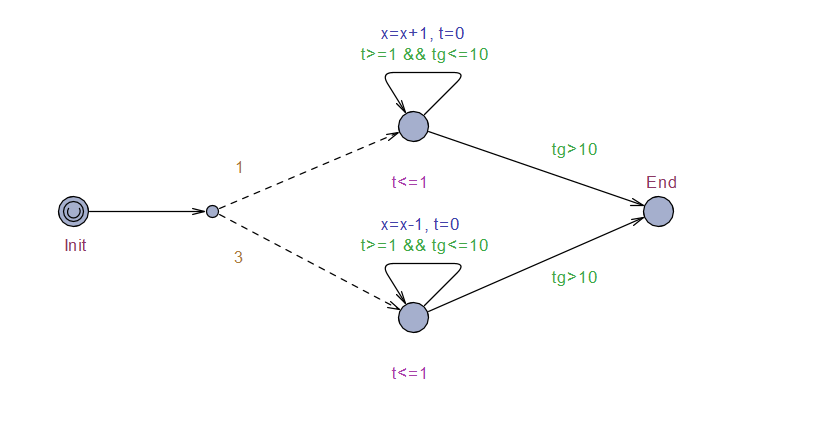
\includegraphics[scale=0.28]{./pictures/model_comparison/uppaal_model_labels.png}
	\caption{Learned Model}
\end{figure}

}
\only<3>{
	\tiny
	Then we perform a simultaneous \textit{breadth-first-search} and compare the functionalities and time constraints of locations against each other. 
%\begin{figure}[h]
%	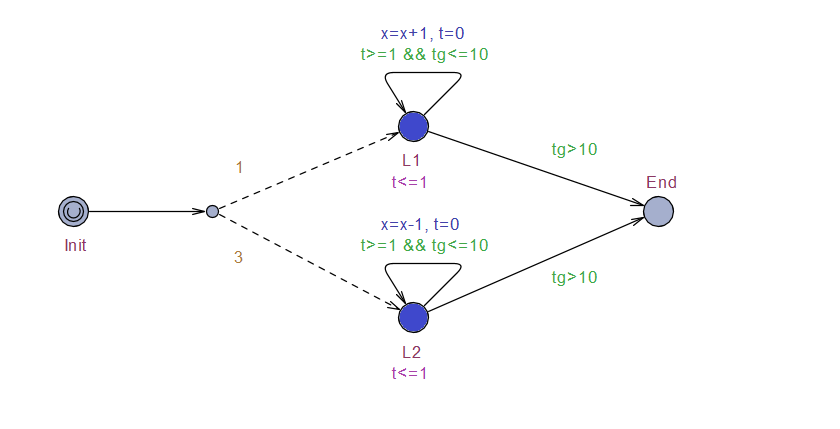
\includegraphics[scale=0.4]{./pictures/model_comparison/uppaal_model_bfs_2.png}
%	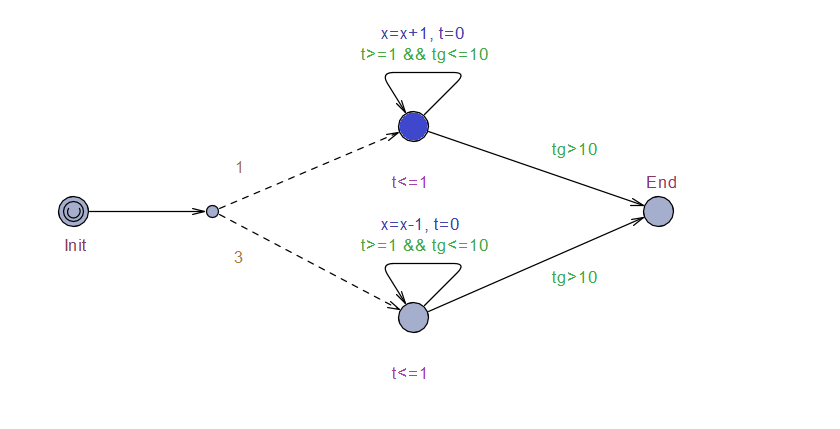
\includegraphics[scale=0.4]{./pictures/model_comparison/uppaal_model_bfs_1.png}
%\end{figure}
\begin{figure}
	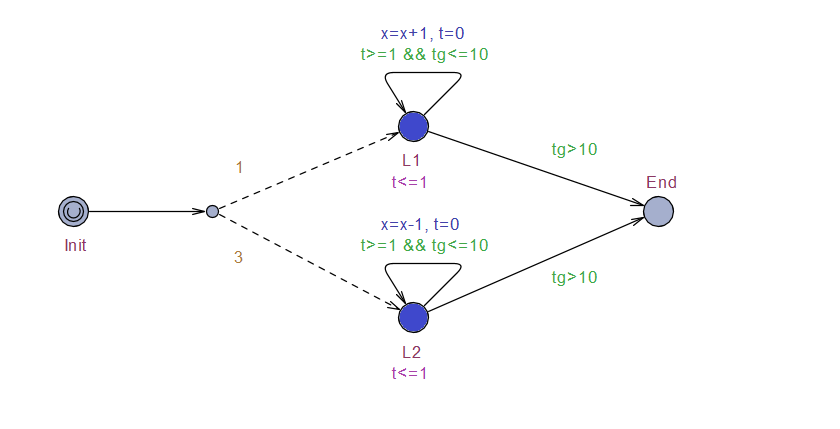
\includegraphics[scale=0.28]{./pictures/model_comparison/uppaal_model_bfs_2.png}
	\caption{Observed Model}
\end{figure}
\begin{figure}
	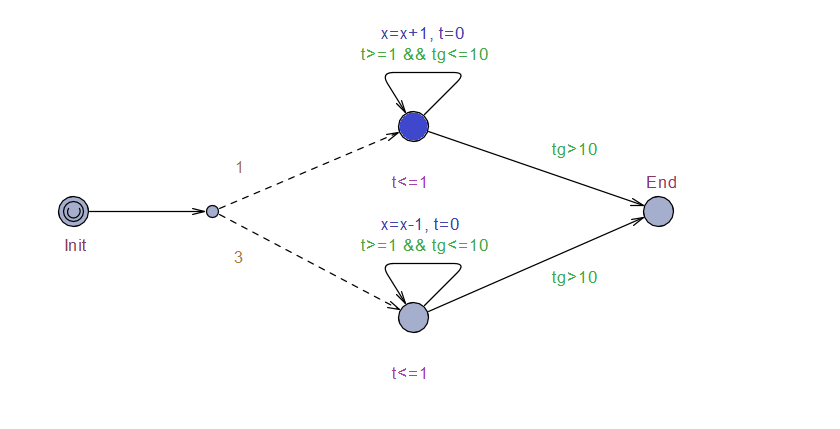
\includegraphics[scale=0.28]{./pictures/model_comparison/uppaal_model_bfs_1.png}
	\caption{Learned Model}
\end{figure}
}
\only<4>{
	\tiny
	Finally, we match the closest locations, based on their functionalities and time constraints. 
%	\begin{figure}[h]
%	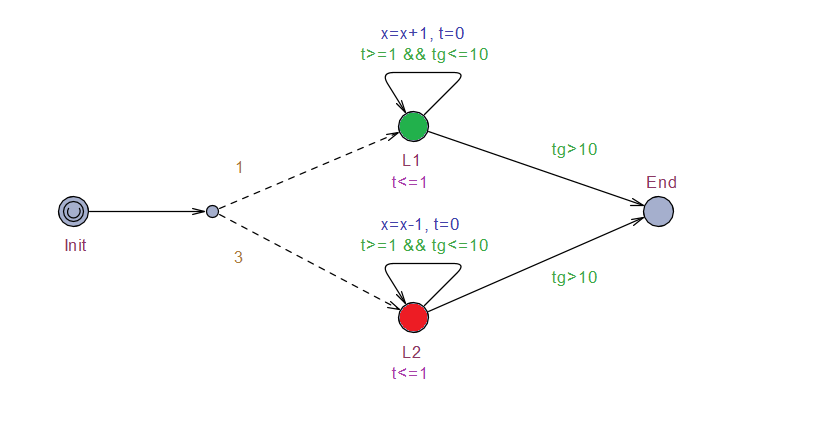
\includegraphics[scale=0.4]{./pictures/model_comparison/uppaal_model_bfs_match_2.png}
%	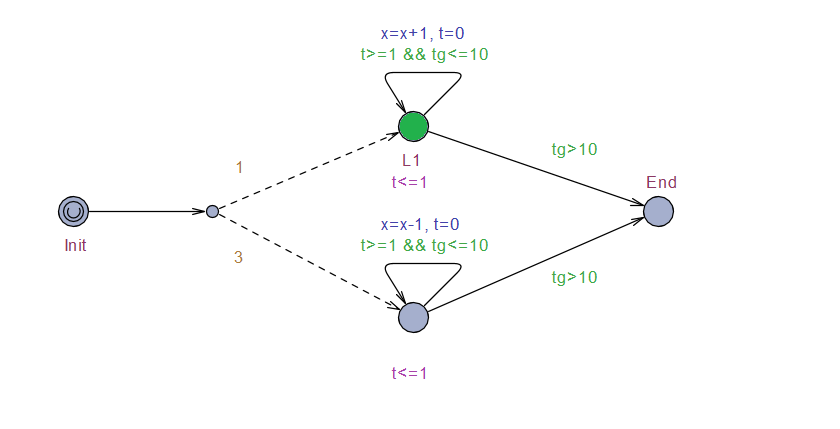
\includegraphics[scale=0.4]{./pictures/model_comparison/uppaal_model_bfs_match_1.png}
%\end{figure}
\begin{figure}
	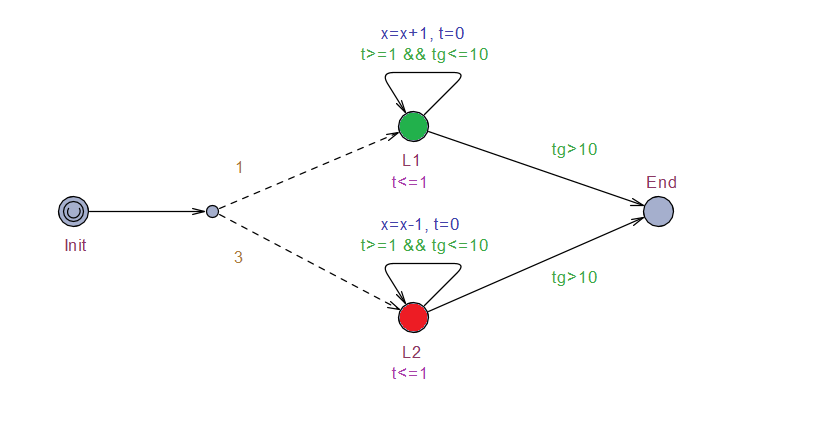
\includegraphics[scale=0.28]{./pictures/model_comparison/uppaal_model_bfs_match_2.png}
	\caption{Observed Model}
\end{figure}
\begin{figure}
	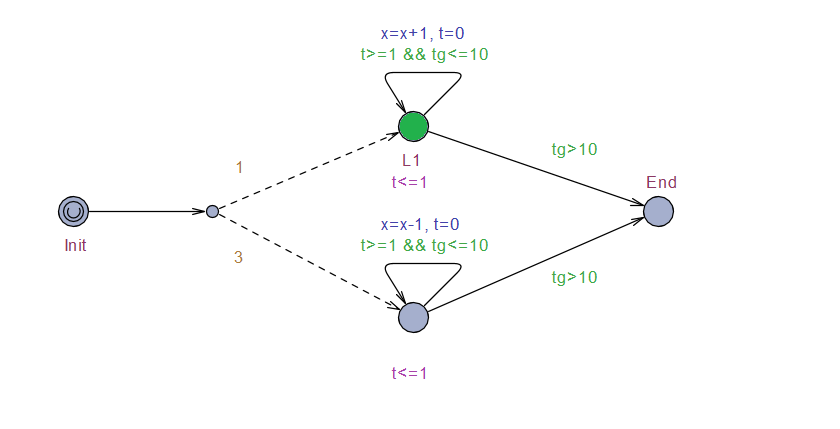
\includegraphics[scale=0.28]{./pictures/model_comparison/uppaal_model_bfs_match_1.png}
	\caption{Learned Model}
\end{figure}
}
\end{center}
%
\end{frame}

\begin{frame}
\frametitle{Automata Representation as Graphs}
\begin{center}
	\begin{figure}
		\includegraphics[scale=0.35]{./pictures/uppaal_model_example.png}
		\caption{UPPAAL Automaton}
	\end{figure}
	\begin{figure}
		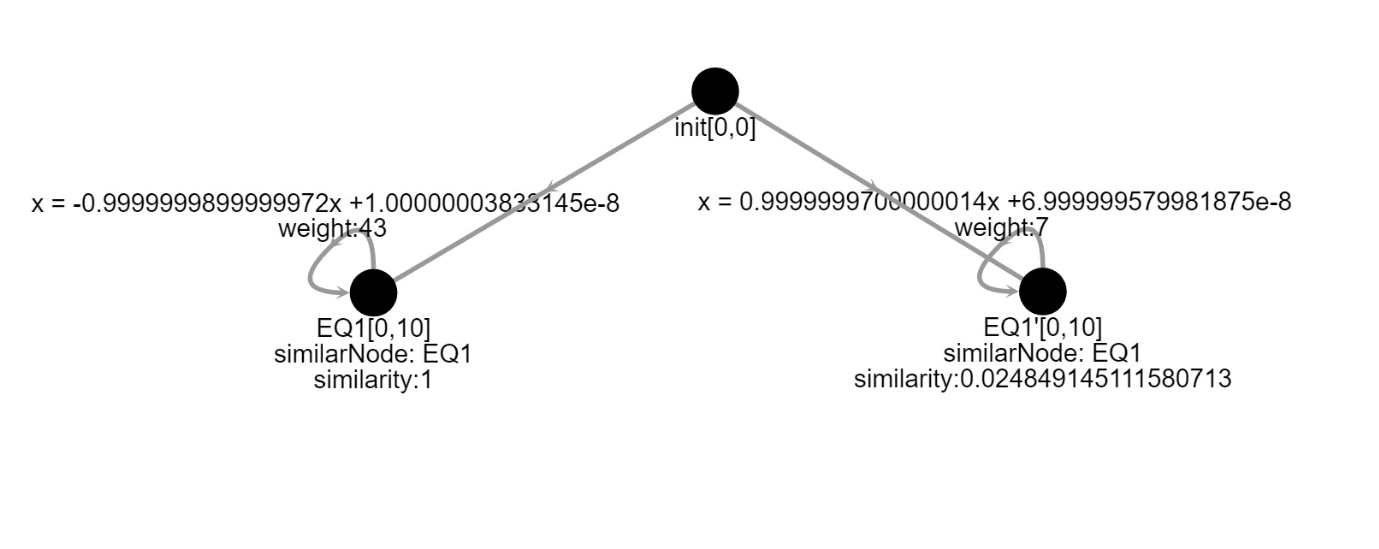
\includegraphics[scale=0.23]{./pictures/experiment_branchedModel_10_times.png}
		\caption{Graph Automaton}
 	\end{figure}
\end{center}
\end{frame}

\section{Implementation}
\begin{frame}
\frametitle{Implementation}
\begin{figure}[h]
	\only<1>{
		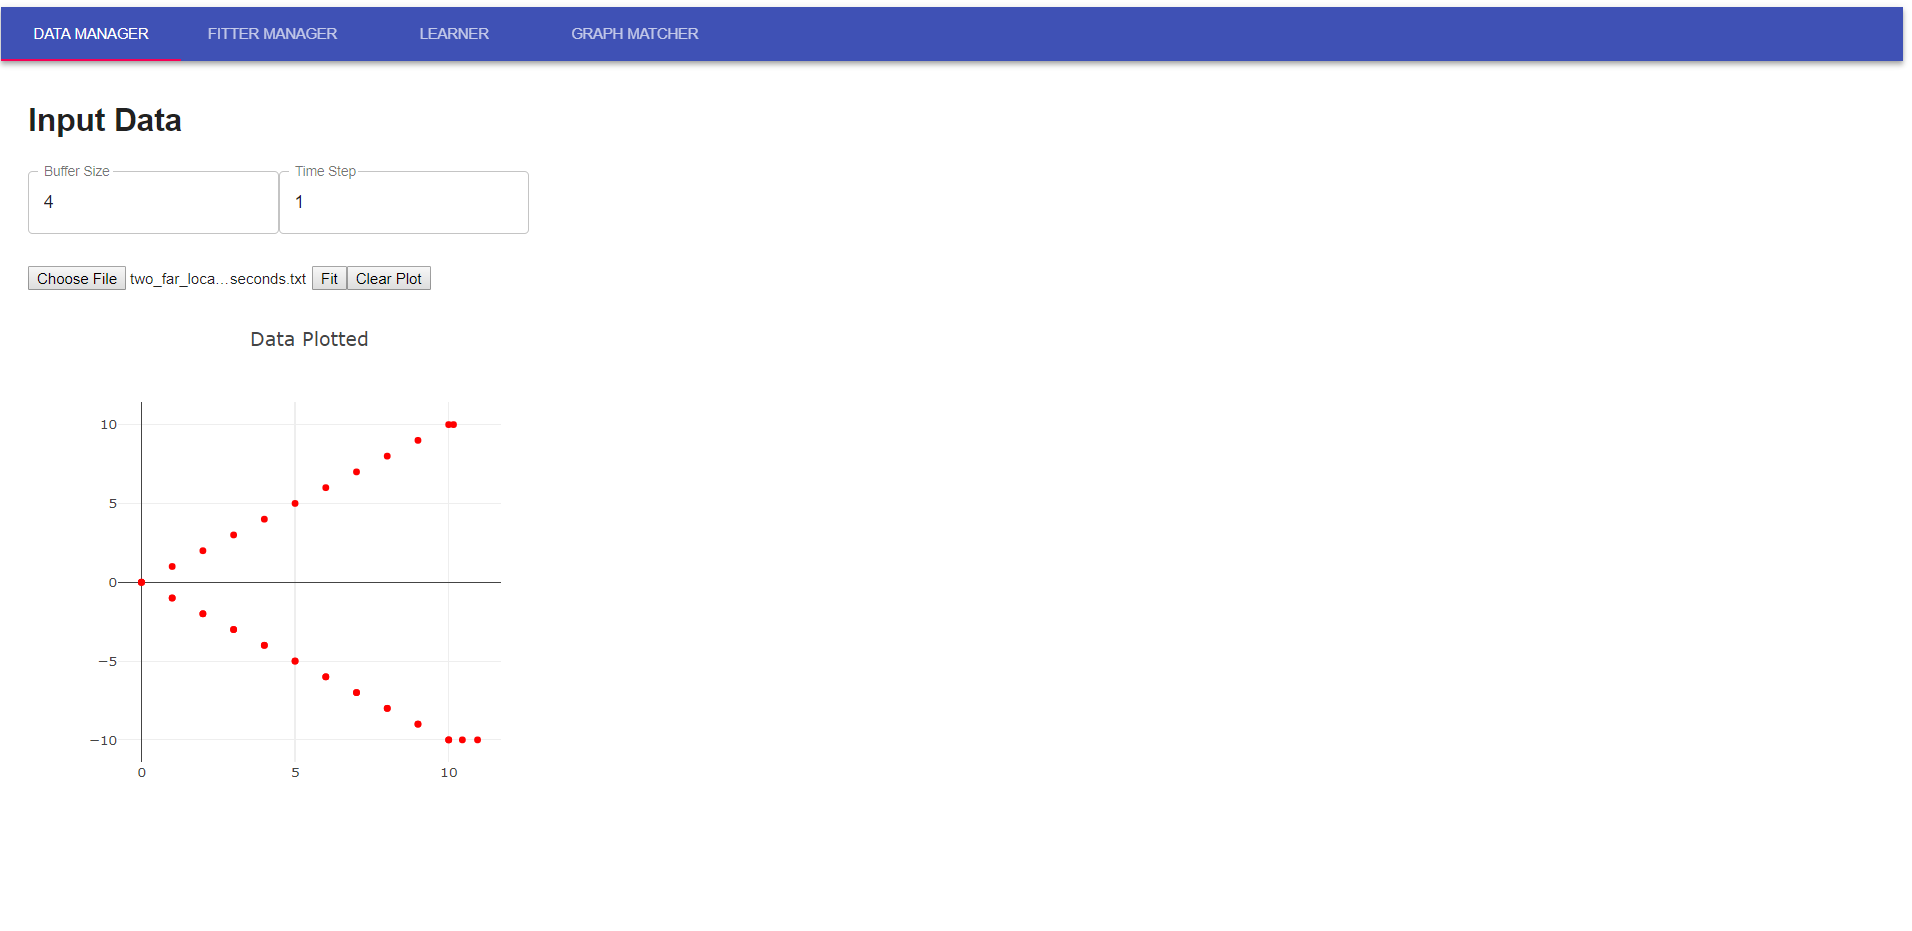
\includegraphics[scale=0.3]{./pictures/implementation/data_manager.png}
		\caption{Data Manager}
	}
	\only<2>{
	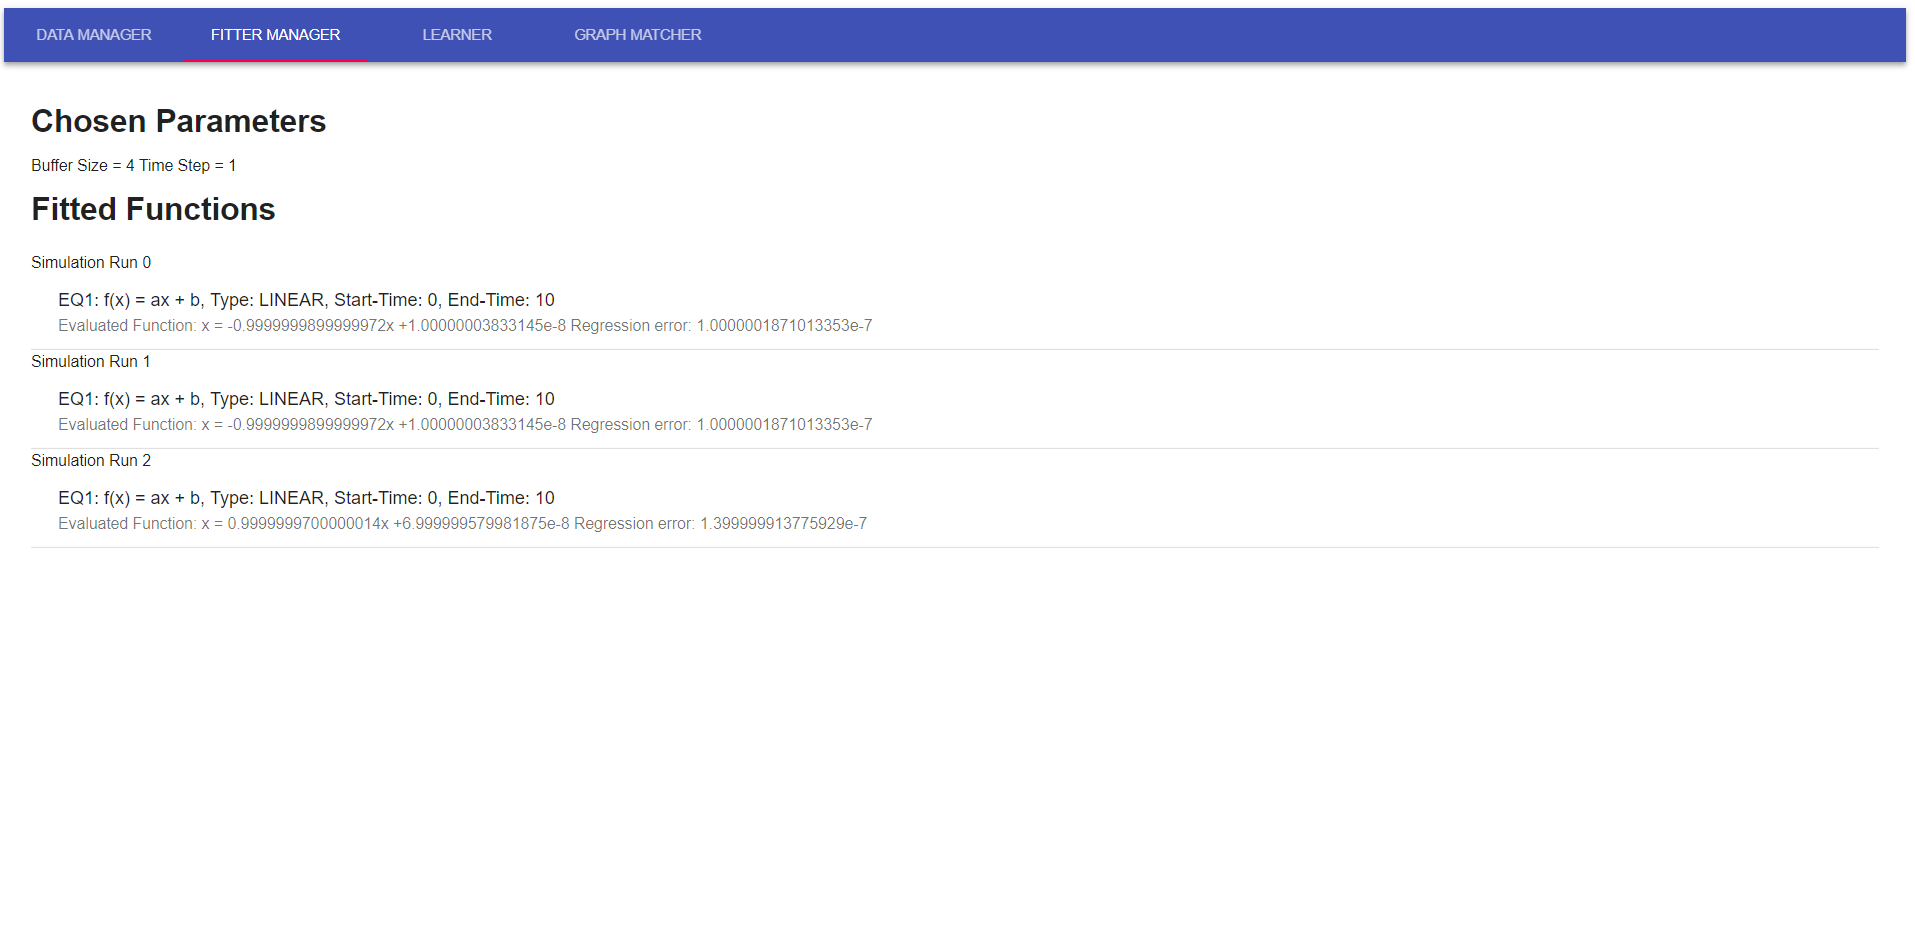
\includegraphics[scale=0.3]{./pictures/implementation/fitter_manager.png}
	\caption{Fitter Manager}
}
\only<3>{
	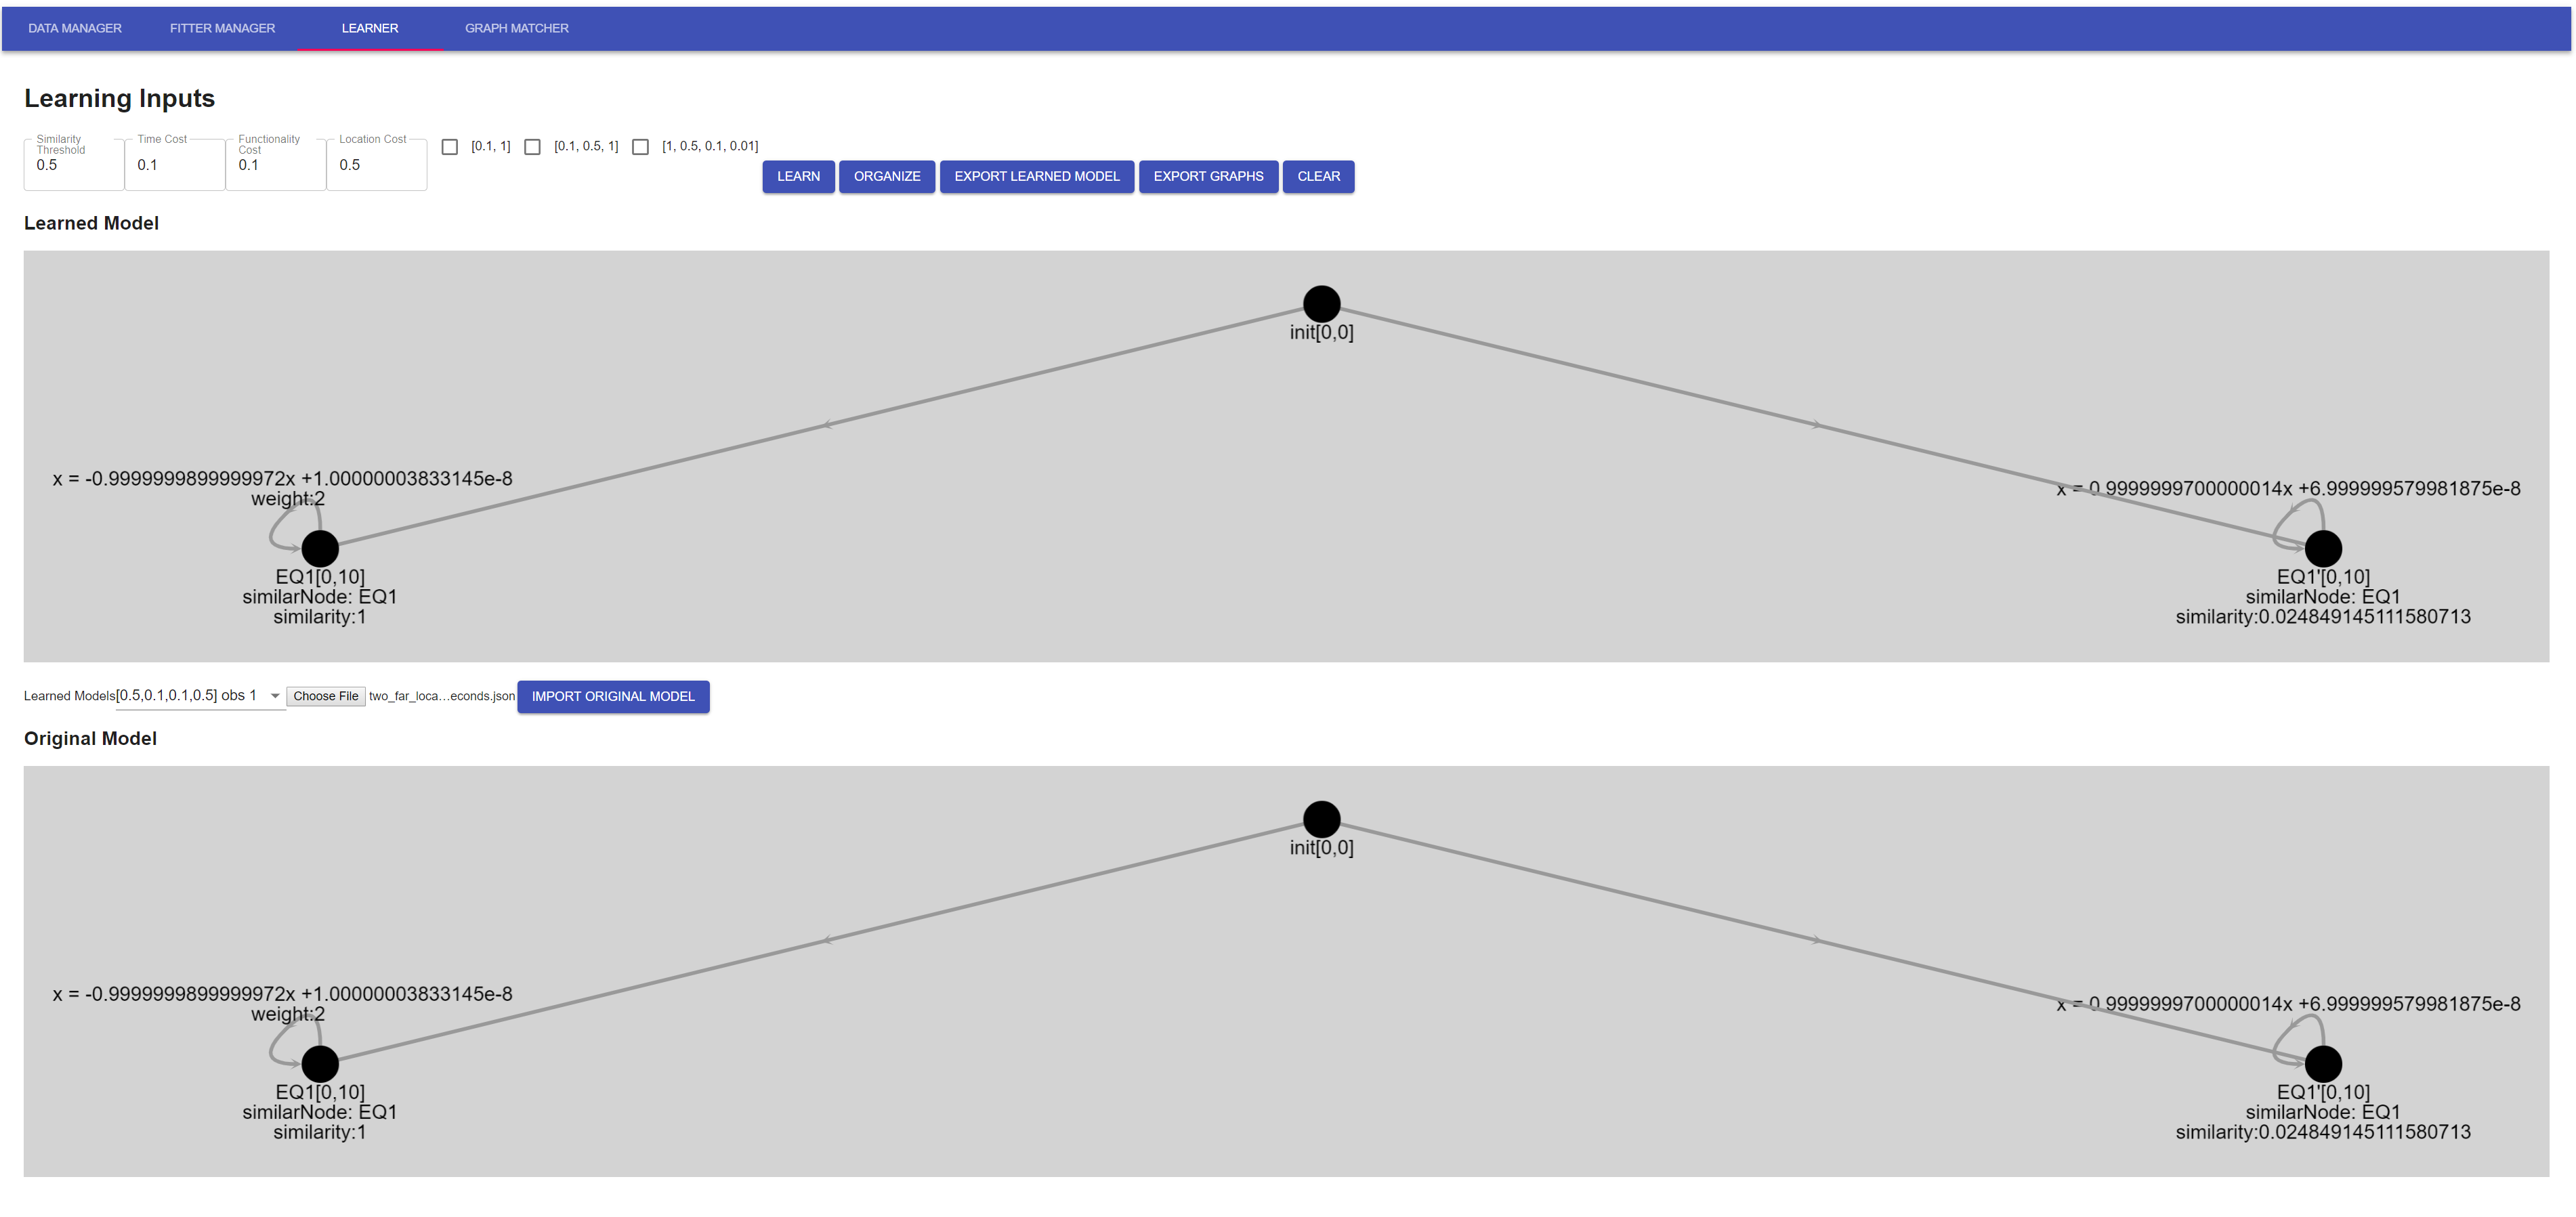
\includegraphics[scale=0.15]{./pictures/implementation/learner.png}
	\caption{Learner}
}
\only<4>{
	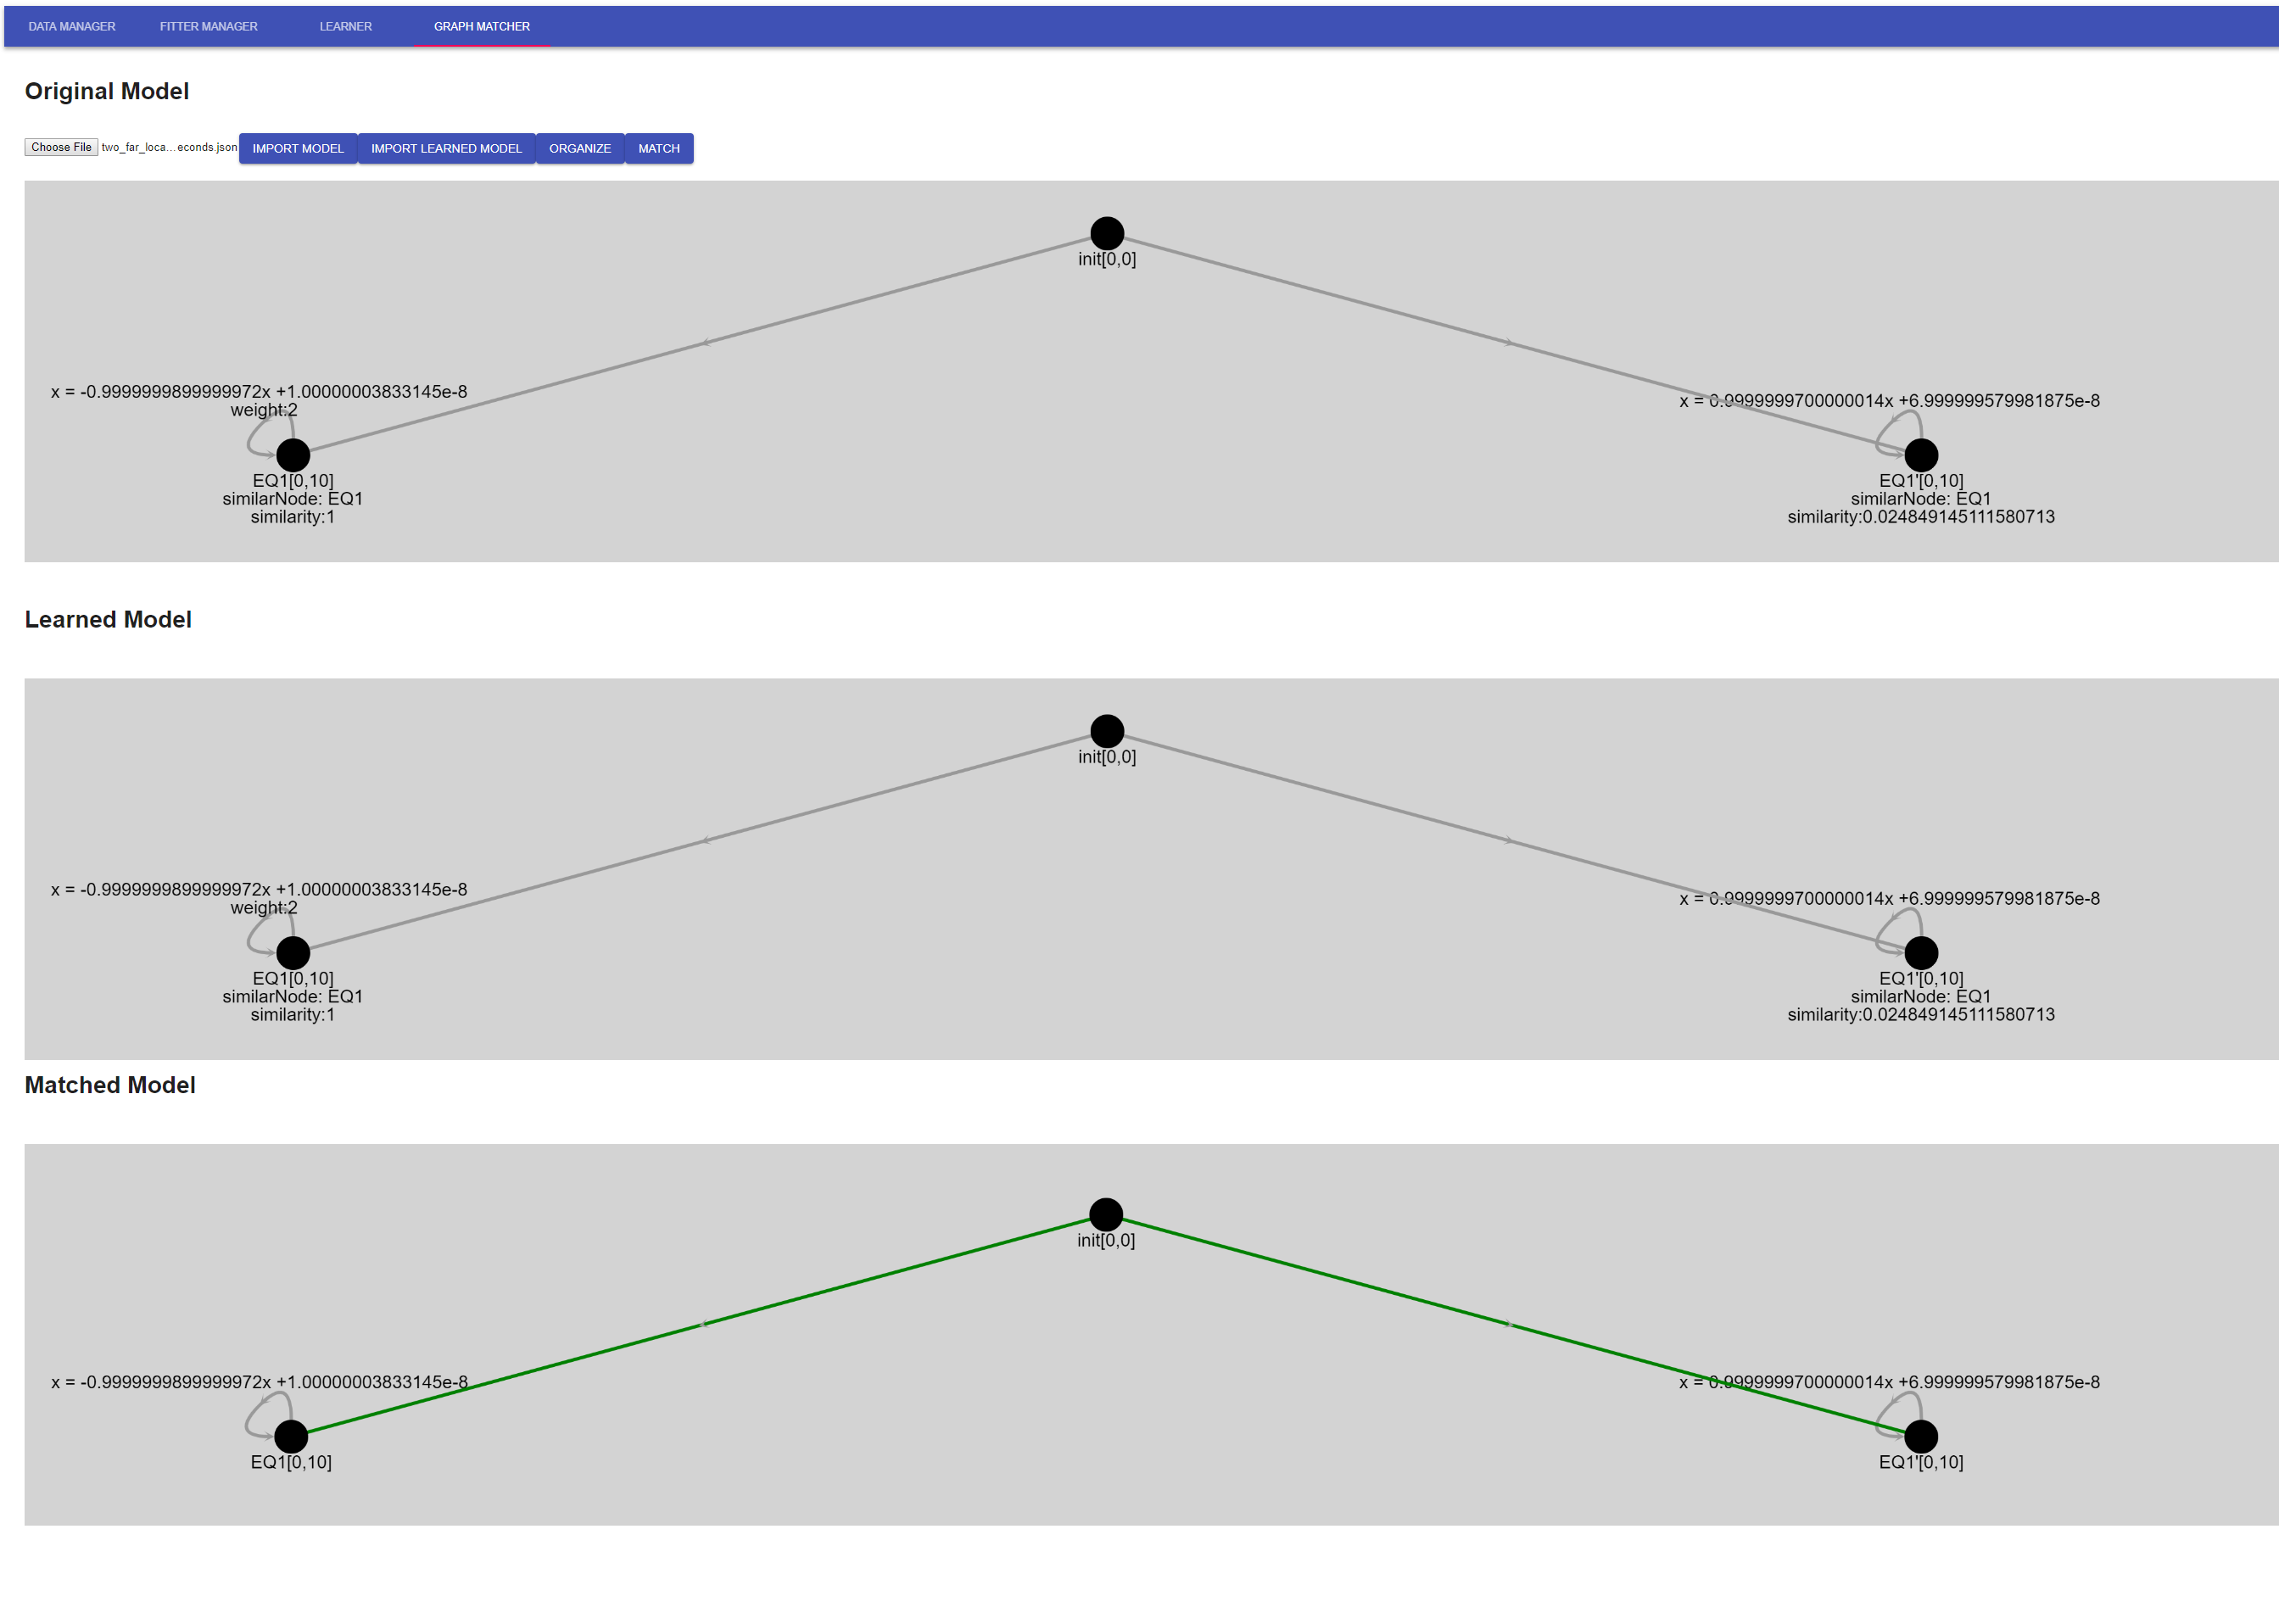
\includegraphics[scale=0.2]{./pictures/implementation/matcher.png}
	\caption{Graph Matcher}
}
\end{figure}
\end{frame}

\section{Experiments}
\begin{frame}
\frametitle{Experiments}
\begin{itemize}
	\item In the following experiments, we chose the values of 0.1, 0.5 and 1 as the possible values for the parameters of the incremental learning algorithm (\textit{similarity threshold}, \textit{functionality cost}, \textit{time cost}, \textit{addition cost}). 
	\item Each model was learned with 81 different combinations, restricted by the previously mentioned set of values. 
\end{itemize}
\end{frame}
\begin{frame}
\frametitle{Experiment 1 }
\scriptsize
	\begin{itemize}
		\item For these experiments, all of the combinations allowed the algorithm to successfully learned the two observed models. 
		\item Every location has a very different functionality. 
		\item Perfect learning was possible because the \textit{similarity threshold} could always distinguish the functionality of each location and because the models are not complex or ambiguous.  
	\end{itemize}

	\begin{figure}[h]
		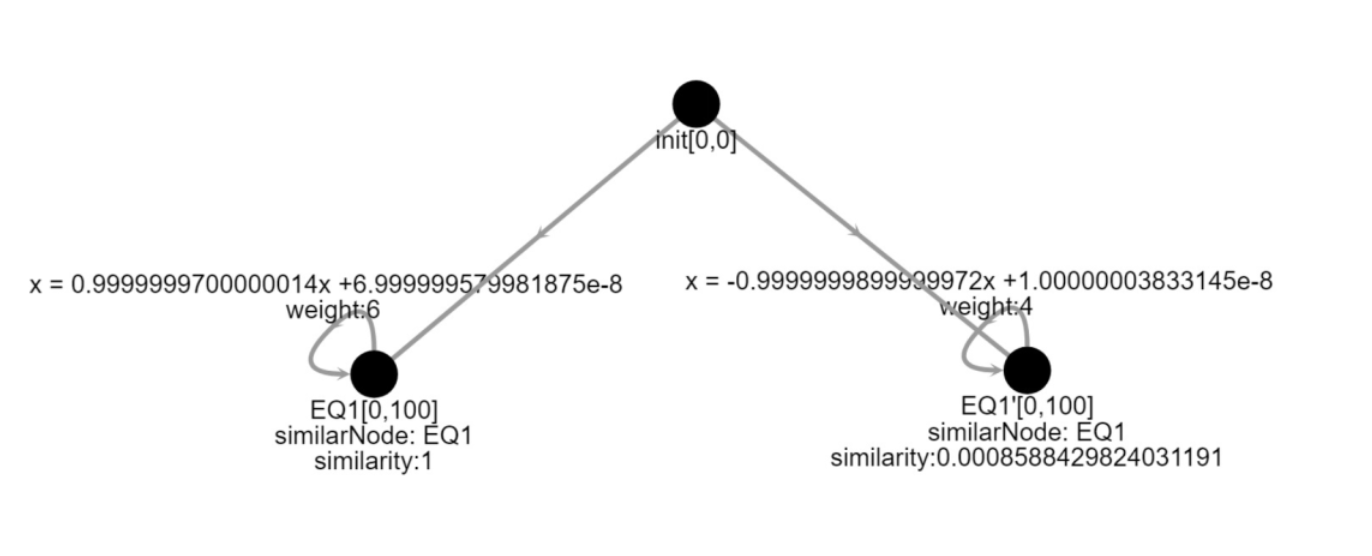
\includegraphics[scale=0.2]{./pictures/experiment_branchedModel.png}
		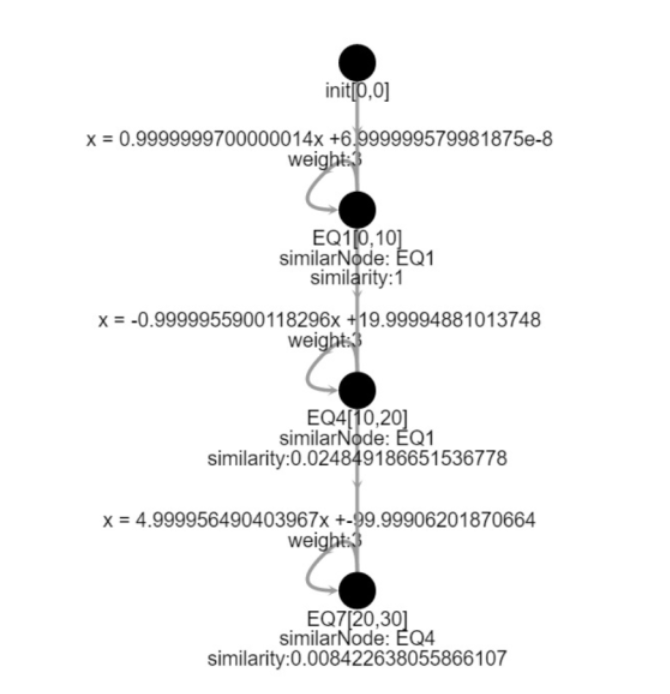
\includegraphics[scale=0.3]{./pictures/experiment_sequentialModel.png}
		\caption{Observed Models}
	\end{figure}
\end{frame}

\begin{frame}
\frametitle{Experiment 2 }
\scriptsize
\begin{itemize}
	\item The complexity of this model was increased by combining the previous models in one, along with extra locations with very close functionalities. 
	\item At the end, 63 out of 81 combinations could match 54\% of the observed model, 6 matched 70\%, and only 12 combinations could match it by 100\%. 
\end{itemize}
\begin{center}
	\begin{figure}
		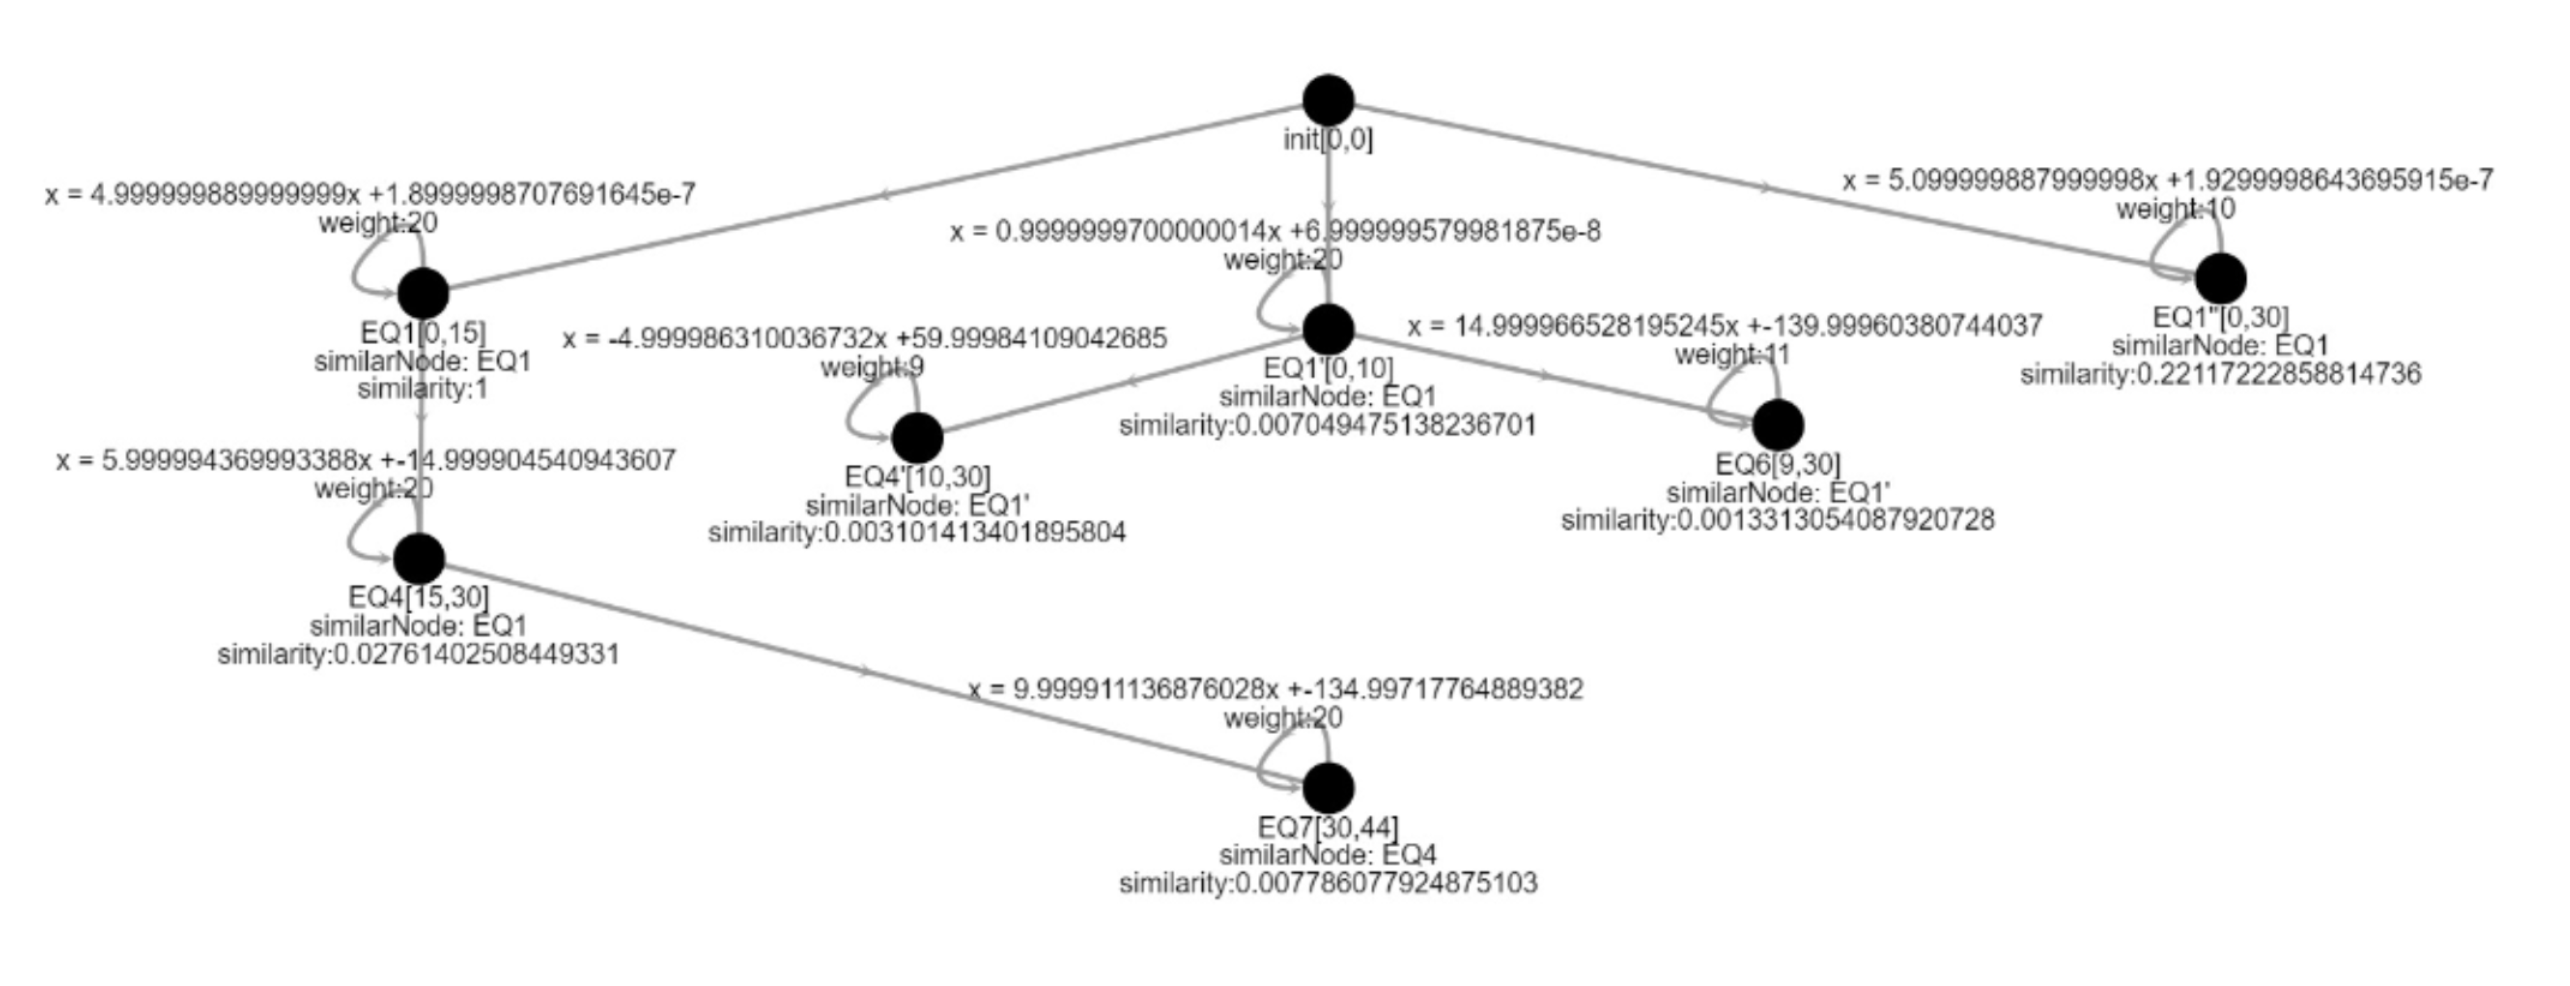
\includegraphics[scale=0.22]{./pictures/experiment_complexModel.png}
		\caption{Observed Model}
	\end{figure}
\end{center}
\end{frame}

\begin{frame}
\frametitle{Experiment 2 - Incremental Learning Progress }
\scriptsize
\begin{itemize}
	\item The model was simulated 50 times.
	\item The x-axis represents the number of observations. 
	\item The y-axis represents the similarity between the observed model and the learned model. 
	\item The legends represent the set of combinations.  
\end{itemize}
\begin{center}
	\begin{figure}
		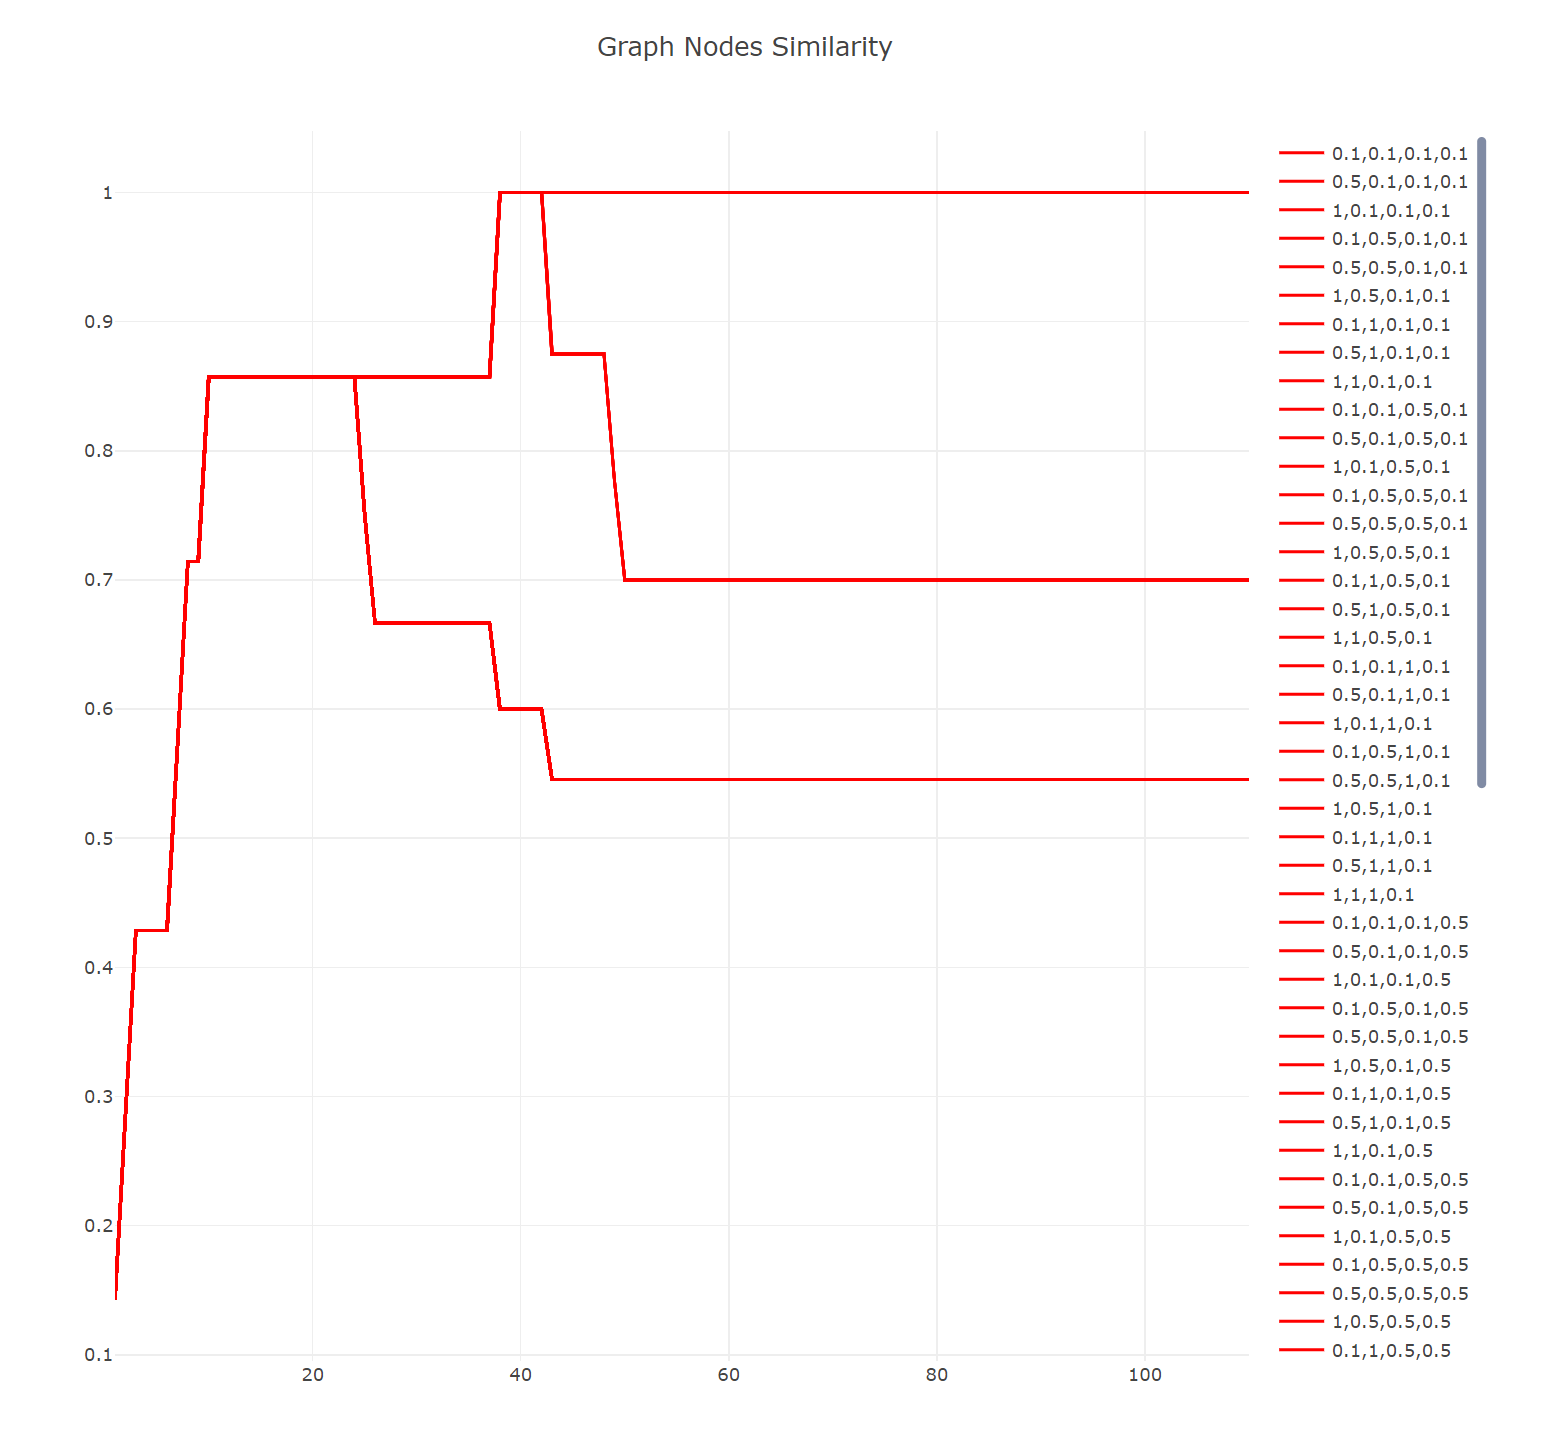
\includegraphics[scale=0.2]{./pictures/complex_experiment_similarities.png}
%		\caption{Observed Model}
	\end{figure}
\end{center}
\end{frame}

\begin{frame}
\frametitle{Experiment 2 - Analysis }
\scriptsize
\begin{itemize}
	\item Some locations have very similar functionalities and time constraints. 
	\item Sometimes the simulation data was not sufficient for the tool to fit the exactly same equation. 
	\item Very extreme cases of the cost function forced the learner to identify any miscalculation or noise from the observations as new functionalities, which sometimes was never the case. 
\end{itemize}
\begin{center}

\end{center}
	\begin{figure}
	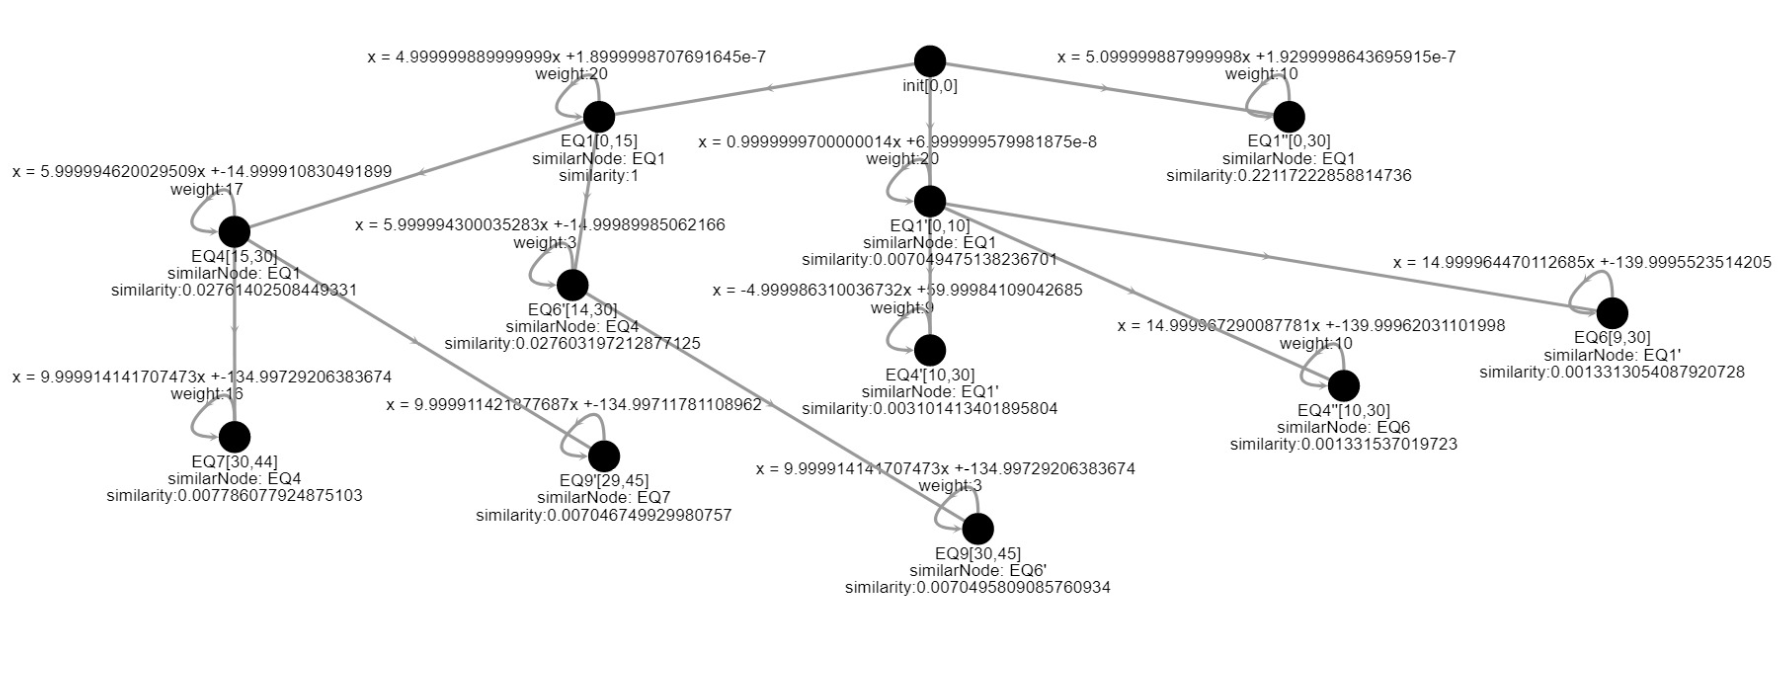
\includegraphics[scale=0.3]{./pictures/learnedModel_worse_experiment.png}
	\caption{Learned Model With Extra Locations}
\end{figure}

\end{frame}

\section{Conclusion and Future Work}
\begin{frame}
\frametitle{Conclusion}
\begin{itemize}
	\item Learning and recreation of models was successful, by analyzing and measuring observations in an incremental fashion, using Euclidean distances and cost functions.
	\item Our approach is able to detect noisy observations, but it was not possible to track the origin of the noise, as there is no interaction with the observed automaton like in active learning. 
	\item Unfortunately, the implementation and concept of this approach is not able to detect optimal combinations on the fly.
\end{itemize}
\end{frame}

\begin{frame}
\frametitle{Future Work}
\begin{itemize}
	\item Automata minimization. Working with a fixed number of locations
	would ensure having a canonical representation of automata, thus reducing complexity
	and ambiguities while learning and matching models.
	\item  We could extend the concept of incremental
	learning to create graph reduction routines which would mainly consist of evaluating the
	cost of eliminating nodes by merging their functionality and time constraints with other
	similar nodes. 
\end{itemize}
\end{frame}

\section{References}
\begin{frame}
\frametitle{References}
\nocite{*}
\renewcommand*{\bibfont}{\tiny}
\bibliographystyle{plain}
\bibliography{sample}
\end{frame}

%\begin{frame}
%\frametitle{References}
%\nocite{*}
%\renewcommand*{\bibfont}{\tiny}
%\bibliographystyle{plain}
%\bibliography{sample2}
%\end{frame}

\section{}
\begin{frame}
\frametitle{Thank you!}

\includegraphics[scale=0.5]{./pictures/q&a.jpg}
\end{frame}

\end{document}